\begin{figure}[htbp]
  \centering
  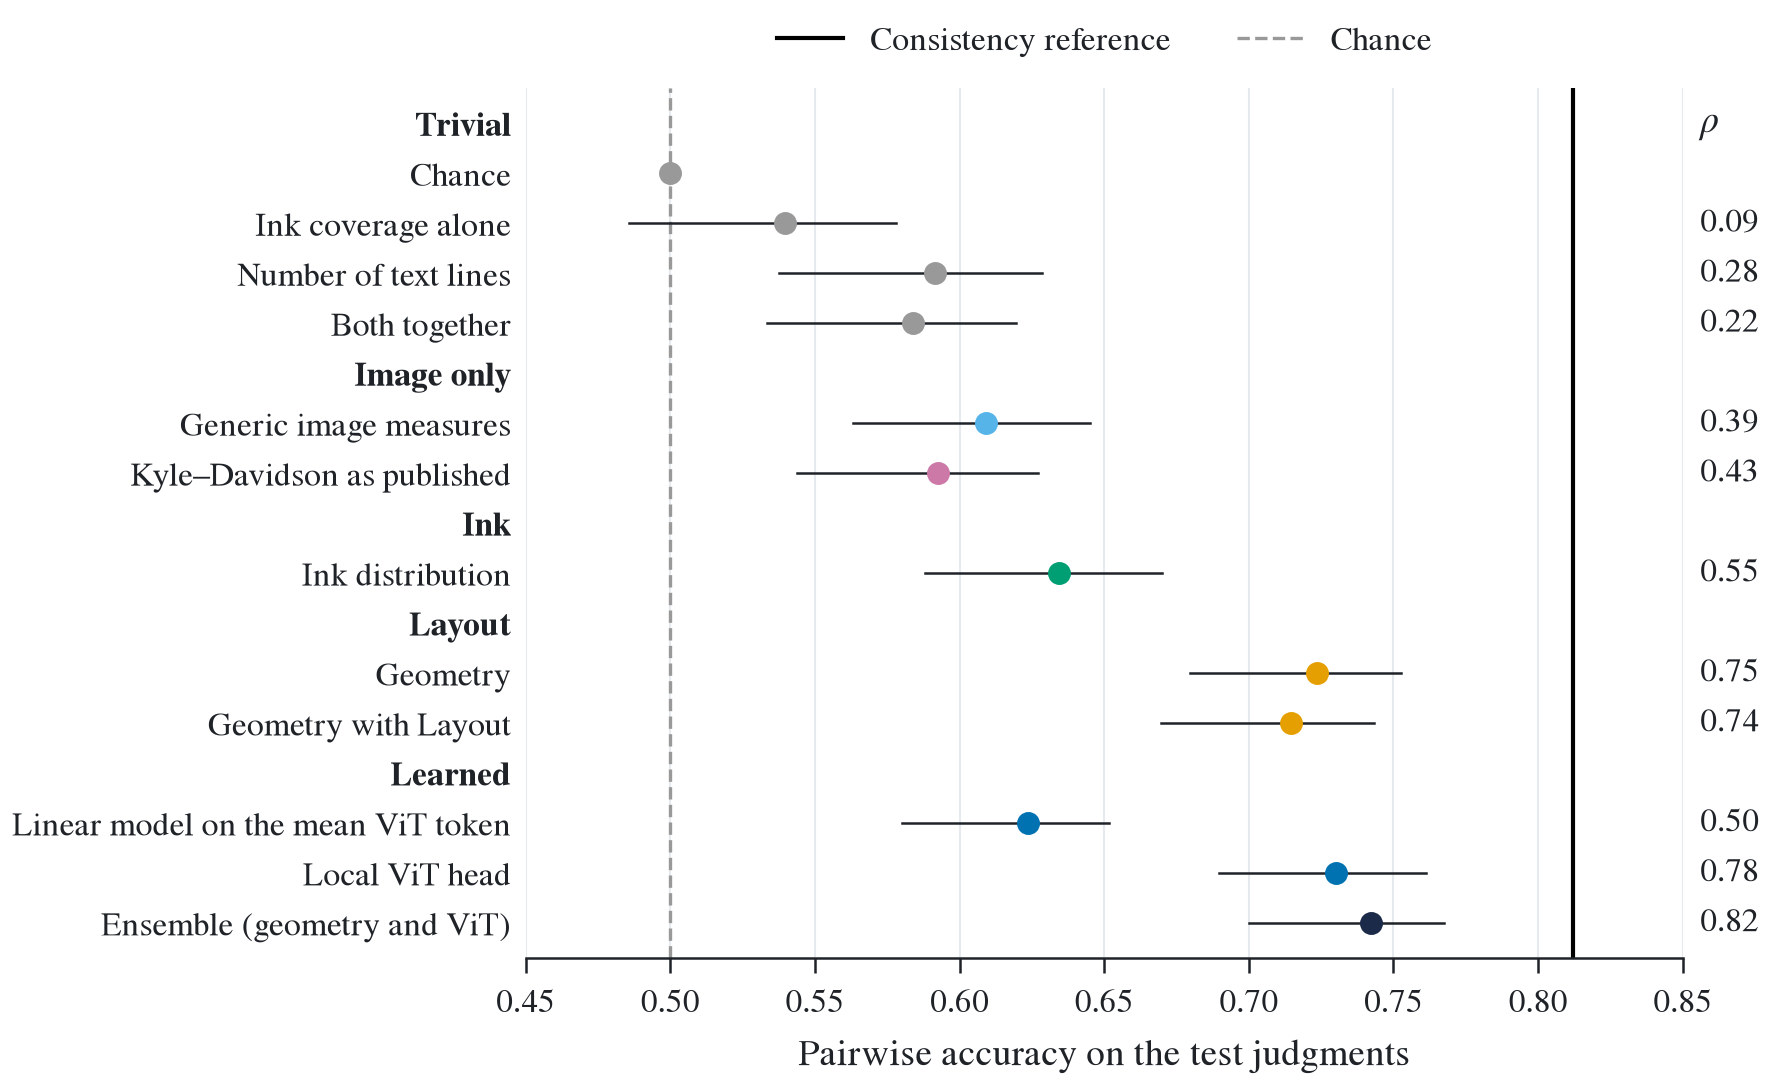
\includegraphics[width=15.00cm]{figures/baselines_by_information.png}
  \caption{What each level of information buys: pairwise accuracy on the test judgments (dots, the mean over the folds, with 95\% intervals from 1,000 resamples of the manuscripts) and Spearman's $\rho$ between the out-of-fold page scores and the Elo scores (right), the methods grouped by the information they need (trivial, image only, ink, layout, learned). The solid line is the consistency reference (0.812), the share of the same test judgments that agree with the final Elo scores; the dashed line is chance. \emph{Ink coverage alone}, the pairwise logistic model on ink coverage alone; \emph{Number of text lines}, the pairwise logistic model on number of text lines alone; \emph{Both together}, the pairwise logistic model on the two trivial measures, ink coverage and number of text lines (2 columns); \emph{Generic image measures}, the pairwise logistic model on the six generic image measures, edge-orientation entropy, MSSC, lossless compressibility, feature congestion, colourfulness and patch-codebook variety (15 columns); \emph{Kyle--Davidson as published}, the pairwise logistic model on the three Kyle--Davidson measures, clutter, symmetry and entropy (7 columns); \emph{Ink distribution}, the pairwise logistic model on the five ink distribution measures, coverage, lacunarity, fragmentation, chromatic share and hue classes (13 columns); \emph{Geometry}, the pairwise logistic model on the 83 geometric features; \emph{Geometry with Layout}, the pairwise logistic model on the 105 geometric and Layout features; \emph{Linear model on the mean ViT token}, the pairwise logistic model on the mean of the page's patch tokens (384 dimensions); \emph{Local ViT head}, the local scoring head on the patch tokens of DINOv2 ViT-S/14 (block 12, 518 pixels on the long edge, the folio crop): an MLP (384--128--1, ReLU, softplus) scoring each patch, the page's score the mean of its patches', trained with RankNet's logistic loss (180 epochs of Adam); \emph{Ensemble (geometry and ViT)}, the mean of the z-scored page scores of \emph{Geometry} and \emph{Local ViT head}. Each method is evaluated by 10-fold cross-validation repeated 10 times, each manuscript's pages in one fold; a fold tests the judgments between two of its pages.}
  \label{fig:baselines_by_information}
\end{figure}
